\section[4]{Experiments}

\begin{frame}{Environment : Input data scenario}
	A traffic model from real Twitter data related to COVID pandemic

    \begin{figure}[!ht]
        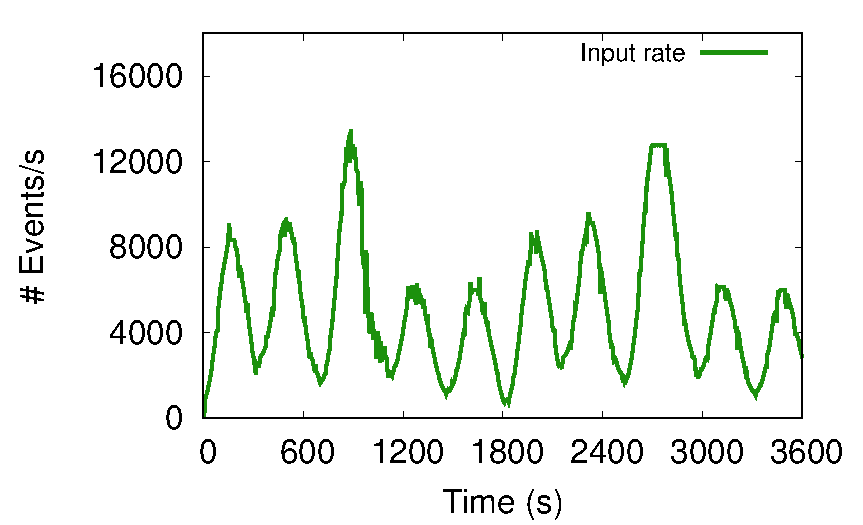
\includegraphics[width=0.75\textwidth]{images/exp/Dataset-TwitterSmoothed.pdf}
        %\caption{Traffic shape of Covid Twitter dataset.}
    \end{figure}
\end{frame}

\begin{frame}{Environment : Application}
	Twitter linear app to classify tweets
	\begin{figure}
		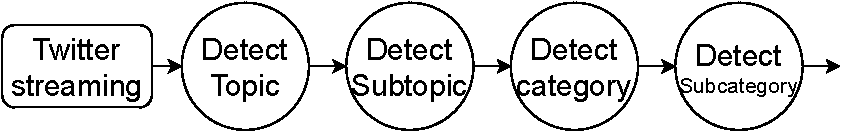
\includegraphics[width=0.9\textwidth]{images/exp/App-Twitter-Linear-1.pdf}
	\end{figure}
\end{frame}

\begin{frame}{Environment : Infrastructure}
	Google Cloud Platform as infrastructure for the deployment

	\begin{figure}
		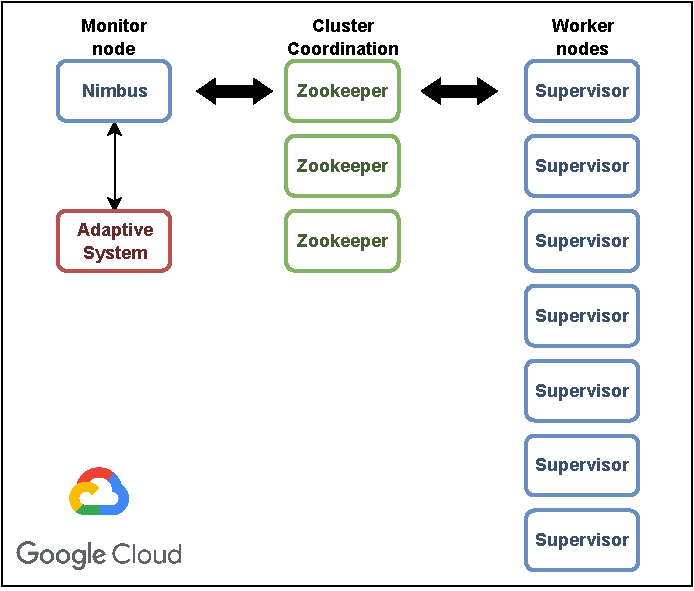
\includegraphics[width=0.75\textwidth]{images/exp/GCP-2.pdf}
	\end{figure}
\end{frame}

\begin{frame}{Evaluation metrics}
	\textit{Saved nodes {\tiny [\cite{LombardiABQ18}]}}
        \begin{itemize}
            \item Proportion
of resources saved with respect to a statically over-provisioned configuration
		 \end{itemize}
	\textit{Throughput degradation {\tiny [\cite{LombardiABQ18}]}}
		 \begin{itemize}
            \item Difference between the input rate and the output rate
         \end{itemize}
	\textit{Latency}
		 \begin{itemize}
         	\item Average time taken by an event between the moment it enters and leaves the SPS
         \end{itemize}
	\textit{Difference in the number of processed events}
		 \begin{itemize}         
            \item Difference between the total number of processed events and the total number of received events
        \end{itemize}
\end{frame}

